% Definição do tamanho da letra, folha e estilo.
\documentclass[12pt, a4paper]{article}

% Definição de pacotes.
%% Padrão UTF-8.
%% Texto brasileiro.
%% Identação dos parágrafos.
%% Adição de imagens.
%% Geometria da página de acordo com a ABNT.
\usepackage[utf8]{inputenc}
\usepackage[brazil]{babel}
\usepackage{indentfirst}
\usepackage{graphicx}
\usepackage{subfigure}
\usepackage{float}
\usepackage{geometry}
\geometry{a4paper, left = 3cm, right = 3cm, top = 3cm, bottom = 3cm}

% Numeração da página.
\pagenumbering{arabic}

% Path das imagens.
\graphicspath{{./img/}}

\title{\textbf{Protocolo Snooping}}
\author{
	Guimarães, João Guilherme M.\\
	\texttt{joaog95@live.com}
}
\date{22 de novembro de 2019}

\begin{document}
	% Escrever o título, autor e data.
	\maketitle
	
	% Espaçamento vertical
	\vspace{1.5cm}
	
	\section{Introdução}
	
	\par Em sistemas com memória compartilhada em que os processadores fazem uso de caches, é necessário manter consistência dos dados armazenados, para facilitar este processo, foi definido o protocolo Snooping, que consiste na utilização de um barramento para envio e recebimento de mensagens entre os processadores. A estrutura do processo de comunicação pode ser visualizado na imagem abaixo.
	
	\vspace{\baselineskip}
	
	\begin{figure}[H]
		\centering
		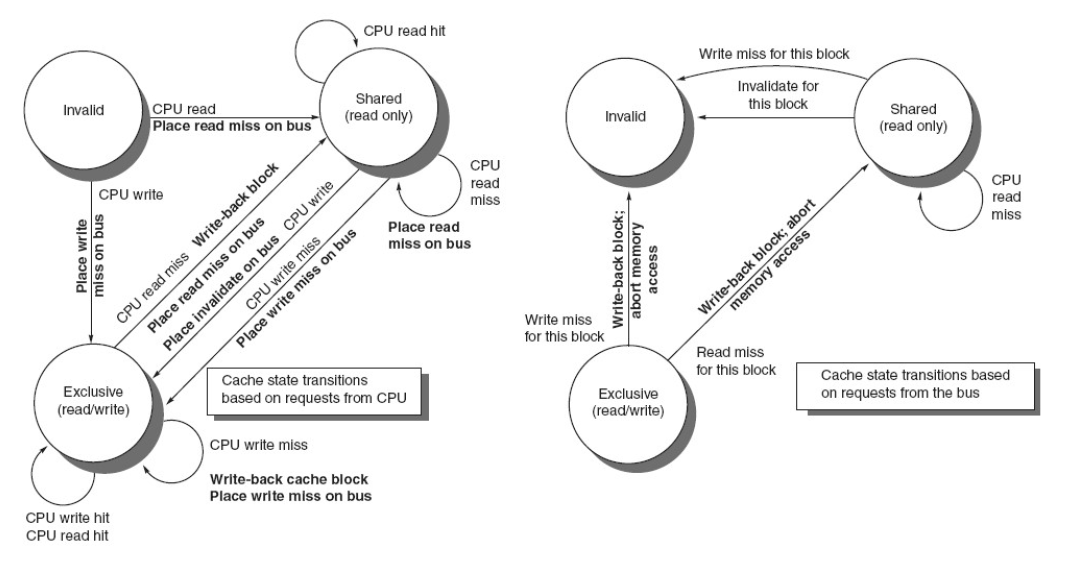
\includegraphics[width=15.3cm]{./protocolo}
		\caption{Protocolo Snooping}
		\label{fig: protocolo Snooping}
	\end{figure}
	
	\section{Objetivos}
	
	\par Implementação do protocolo Snooping definido na figura \ref{fig: protocolo Snooping}, com estrutura \textit{write-back}.
	
	\section{Material}
	
	\par Para realização desta prática, foi utilizado os seguintes equipamentos e softwares:
	
	\begin{itemize}
		\item ModelSim 10.1d;
		\item Quartus 13.0sp1;
		\item FPGA EP2C35F672C6 e
		\item Kernel Linux / SO Deepin 15.11.
	\end{itemize}
	
    \section{Desenvolvimento}
    
	\par Para facilitar na implementação do protocolo Snooping, foi criado dois projetos, um referente ao envio de mensagens e outro para escutar as alterações no barramento. A partir disso, foi definido as seguintes constantes para envio de mensagens no barramento.
	
	\begin{itemize}
		\item RM - read miss;
		\item RH - read hit;
		\item WM - write miss e
		\item WH - write hit.
	\end{itemize}

	\section{Simulação}
	
	\par Com a criação de dois projetos distintos para o protocolo Snooping, suas simulações foram separadas, sendo a primeira a seguir referente ao processo de escrita no barramento (máquina de estados à esquerda da figura \ref{fig: protocolo Snooping}) e a segunda, o processo de escutar as mensagens do barramento (máquina da direita da mesma figura).
	
	\subsection{Processo de envio de mensagens}
	
	\begin{figure}[H]
		\centering
		\subfigure[Inválido para Compartilhado (RM)]{
			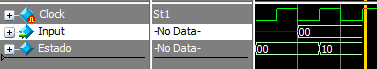
\includegraphics{writing/invalid_to_shared}
		}
		\subfigure[Inválido para Modificado (WM)]{
			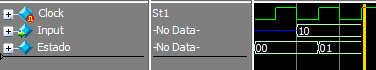
\includegraphics{writing/invalid_to_exclusive}
		}
		\subfigure[Modificado para Compartilhado (RM)]{
			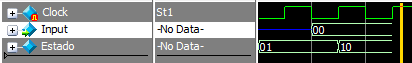
\includegraphics{writing/exclusive_to_shared}
		}
		\subfigure[Permanecendo Modificado (WH)]{
			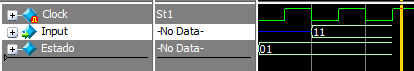
\includegraphics{writing/exclusive_to_exclusive}
		}
		\caption{Mudança de estados}
		\label{writing}
	\end{figure}
	
	
	\subsection{Processo de leitura do barramento}
	
	\begin{figure}[H]
		\centering
		\subfigure[Modificado para Compartilhado (RM)]{
			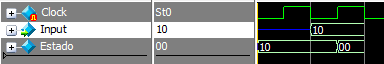
\includegraphics{listening/shared_to_invalid}
		}
		\subfigure[Compartilhado para Inválido (WM)]{
			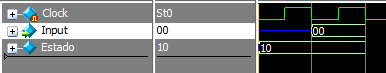
\includegraphics{listening/shared_to_shared}
		}
		\subfigure[Compartilhado para Compartilhado (RM)]{
			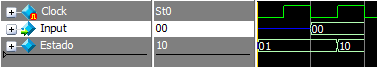
\includegraphics{listening/exclusive_to_shared}
		}
		\caption{Mudança de estados}
		\label{listening}
	\end{figure}
	

	\section{Conclusão}
	
	\par Com a execução desta prática, foi possível reforçar os conhecimentos do Protocolo Snooping e entender na prática, o desenvolvimento do código de uma máquina de estados em Verilog.

\end{document}
	